\documentclass{beamer}
\usepackage{beamerThemeLogic}
% \usetheme{Warsaw}
\usetheme{IrvineMath}

\usepackage{amsmath, amssymb}
\usepackage{physics}
\usepackage{svg}
\usepackage{mathtools}


\usepackage{graphicx}
\graphicspath{{../figures/}}

\usepackage{tikz}
\usetikzlibrary{arrows.meta}
\usetikzlibrary{calc}
\usetikzlibrary{decorations.markings}
\usetikzlibrary{overlay-beamer-styles}

\author{Eli Griffiths}
\title{The Banach Mazur Game}
\subtitle{A Dynamic View of Topological Largeness}
\institute[UCI]{University of California, Irvine}
\date{April 17, 2026}

% \directlua{graph = require("../scripts/graph")}
% \directlua{examples = require("../scripts/data")}

\definecolor{aliceblue}{RGB}{52,101,164}
\definecolor{bobred}{RGB}{180,50,47}
\definecolor{darkgray}{RGB}{60,60,60}
\definecolor{softgreen}{RGB}{34,139,34}
\definecolor{softorange}{RGB}{245,158,11}
\definecolor{targetpurple}{RGB}{124,58,237}

\begin{document}

\maketitle

\begin{frame}{The Game Itself}%
    \begin{center}
        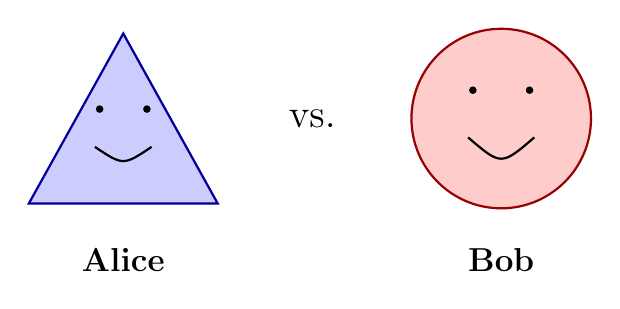
\begin{tikzpicture}[scale=1.2, every node/.style={font=\large}]
            % Alice
            \filldraw[fill=blue!20, draw=blue!60!black, thick]
                (-2,0.4) -- (-3,-1.4) -- (-1,-1.4) -- cycle;
            % eyes
            \fill (-2.25,-0.4) circle (0.04);
            \fill (-1.75,-0.4) circle (0.04);
            % smile
            \draw[thick] (-2.3,-0.8) .. controls (-2,-1.0) .. (-1.7,-0.8);
            \node at (-2,-2.0) {\textbf{Alice}};

            % Bob
            \filldraw[fill=red!20, draw=red!60!black, thick]
                (2,-0.5) circle (0.95);
            % eyes
            \fill (1.7,-0.2) circle (0.04);
            \fill (2.3,-0.2) circle (0.04);
            % smile
            \draw[thick] (1.65,-0.7) .. controls (2,-1.0) .. (2.35,-0.7);
            \node at (2,-2.0) {\textbf{Bob}};

            % middle text
            \node at (0,-0.5) {\Large vs.};
        \end{tikzpicture}
    \end{center}

    \only<2>{
    \begin{center}
        Let $A \subset \R$ be given.
    \end{center}
    }

    \only<3>{
    A \textit{run} of the game is a sequence of open non-empty intervals $U_n$ and $V_n$ such that
    % \[
    %     U_0 \supset V_0 \supset U_1 \supset V_1 \supset \ldots
    % .\]
    \[
        \colorbox{blue!20}{$U_1$}
        \supset
        \colorbox{red!20}{$V_1$}
        \supset
        \colorbox{blue!20}{$U_2$}
        \supset
        \colorbox{red!20}{$V_2$}
        \supset \cdots
    \]
    }


    \only<4>{
    Bob wins if
    \[
        A \cap (U_1 \cap V_1 \cap U_2 \cap V_2 \ldots) = \varnothing
    .\]
    Otherwise Alice wins.
    }
\end{frame}

\begin{frame}<1-3>[label=winning]{Identifying Winning Strategies}
    \only<1-3>{
    What choices of $A$ can Bob always win?

    \pause

    \begin{itemize}[<+->]
        \item $A$ is finite
        \item $A$ is countably infinite
    \end{itemize}
    }

    \only<4->{
    \begin{theorem}[Meager $\Rightarrow$ Strategy]
        If $A$ is meager, then Bob has a winning strategy.
    \end{theorem}
    }

    \only<5>{
    \begin{theorem}[Strategy $\Rightarrow$ Meager]
        If Bob has a winning strategy, then $A$ is meager
    \end{theorem}
    }
\end{frame}

\begin{frame}{Formalizing Strategy}
    \begin{definition}[Strategy]
        A \textbf{strategy} for Bob is a sequence of maps 
        \[
            \sigma_n : (U_0, V_0, \ldots, U_n) \mapsto V_n \subset U_n
        .\]
        A strategy may also be of the form $\sigma_n(U_n) = V_n$, relying on just the last move.
    \end{definition}

    \begin{definition}[Winning Strategy]
        A strategy $\qty(\sigma_n)_{n \in \N}$ for Bob is winning if for any run
        \[
            U_1 \supset V_1 \supset U_2 \supset V_2 \supset \ldots
        \]
        where $\sigma_n(U_1, V_1, \ldots, U_n) = V_n$, it holds that
        \[
            A \cap \bigcap_{n \in \N} U_n = A \cap \bigcap_{n \in \N} V_n = \varnothing
        .\]
    \end{definition}
\end{frame}


\againframe<4-5>{winning}

\begin{frame}{"Proving" the Converse}
    \only<1>{
    \begin{theorem}
        If Bob has a winning strategy, then $|A^c| \geq |\R|$.
    \end{theorem}
    }

    \only<2->{
    \centering
    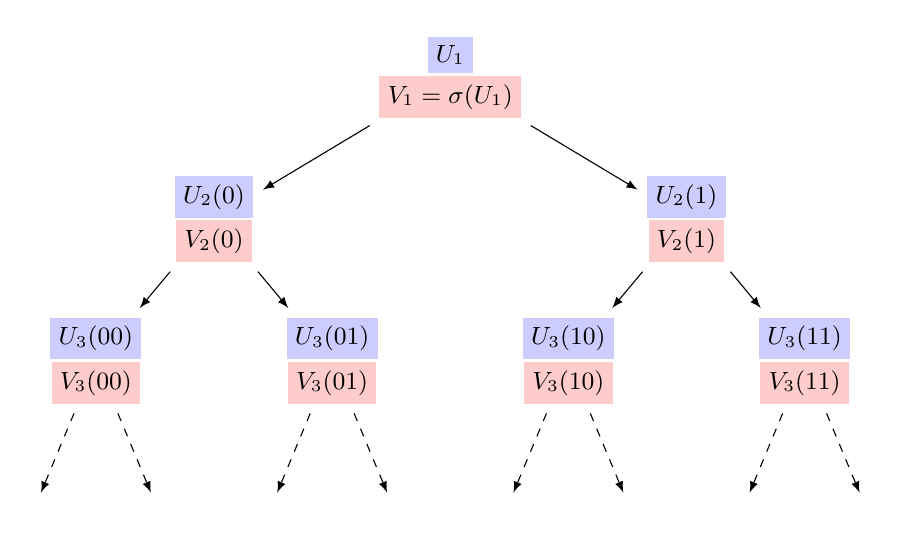
\begin{tikzpicture}[
        level 1/.style={sibling distance=60mm},
        level 2/.style={sibling distance=30mm},
        level 3/.style={sibling distance=15mm},
        level distance=18mm,
        every node/.style={align=center, font=\small},
        edge from parent/.style={draw, -latex}
        ]
        \node[visible on=<2->] {
                \colorbox{blue!20}{$U_1$}\\
                \colorbox{red!20}{$V_1=\sigma(U_1)$}
            }
            child[visible on=<3->] {
                node {
                    \colorbox{blue!20}{$U_2(0)$}\\
                    \colorbox{red!20}{$V_2(0)$}
                }
                child[visible on=<4->] {
                    node {
                        \colorbox{blue!20}{$U_3(00)$}\\
                        \colorbox{red!20}{$V_3(00)$}
                    }
                    child {
                        node {}
                        edge from parent[dashed]
                    }
                    child {
                        node {}
                        edge from parent[dashed]
                    }
                }
                child[visible on=<4->] {
                    node {
                        \colorbox{blue!20}{$U_3(01)$}\\
                        \colorbox{red!20}{$V_3(01)$}
                    }
                    child {
                        node {}
                        edge from parent[dashed]
                    }
                    child {
                        node {}
                        edge from parent[dashed]
                    }
                }
            }
            child[visible on=<3->] {
                node {
                    \colorbox{blue!20}{$U_2(1)$}\\
                    \colorbox{red!20}{$V_2(1)$}
                }
                child[visible on=<4->] {
                    node {
                        \colorbox{blue!20}{$U_3(10)$}\\
                        \colorbox{red!20}{$V_3(10)$}
                    }
                    child {
                        node {}
                        edge from parent[dashed]
                    }
                    child {
                        node {}
                        edge from parent[dashed]
                    }
                }
                child[visible on=<4->] {
                    node {
                        \colorbox{blue!20}{$U_3(11)$}\\
                        \colorbox{red!20}{$V_3(11)$}
                    }
                    child {
                        node {}
                        edge from parent[dashed]
                    }
                    child {
                        node {}
                        edge from parent[dashed]
                    }
                }
            };
    \end{tikzpicture}
    }
    \only<5>{
    \[
        b=(b_1,b_2,\dots)\in\{0,1\}^{\mathbb N}
        \quad\rightsquigarrow\quad
        \bigl(U_n(b_1,\dots,b_n),V_n(b_1,\dots,b_n)\bigr)_{n\ge 1}
    \]
    }

\end{frame}

\begin{frame}{Generalizing the Game}
    Let $X$ be a topological space, with $A \subset X$ and Alice and Bob's set choices being non-empty open sets in $X$. Winning conditions are the same.

    \pause

    \begin{theorem}
        If $A$ is meager, then Bob has a winning strategy.
    \end{theorem}

    \pause

    \begin{definition}[Completely Metrizable]
        $X$ is completely metrizable if there exists a complete metric $d$ on $X$ that induces the topology of $X$; that is, the set of all open $d$-balls generates $X$.
    \end{definition}

    \pause

    \begin{theorem}
        Let $X$ be completely metrizable. If Bob has a winning strategy, then $A$ is meager.
    \end{theorem}
\end{frame}

\begin{frame}{Modifying the Game}

    \begin{definition}[Modified Banach Mazur]
        Alice and Bob similarly choose $U_1 \supset V_1 \supset \ldots$ such that $U_n, V_n \in \tau_X$. Bob wins if
        \[
            \bigcap_{n \in \N} U_n = \bigcap_{n \in \N} V_n = \varnothing
        .\]
        Otherwise Alice wins. Denote this modified game as $BM(X)$.
    \end{definition}
\end{frame}

\begin{frame}{Connection to Baire Spaces}
    \begin{definition}[Baire Space]
        A space $X$ is Baire if for any sequence $U_n$ of dense open sets, $\bigcap U_n$ is dense.
    \end{definition}

    \pause

    \begin{theorem}
        A space $X$ is Baire if and only if Alice has no winning strategy in $BM(X)$.
    \end{theorem}
\end{frame}

\begin{frame}{Why Care?}
    \pause
    \begin{enumerate}[<+->]
        \item Intuition for Topological Size and Baire Spaces
        \item Utility in Proving Results (\href{https://arxiv.org/pdf/2211.00432}{Ex. 1} and \href{https://arxiv.org/pdf/2506.11118}{Ex. 2})
        \item Historical Relevancy
    \end{enumerate}
\end{frame}

\end{document}
